\documentclass[12pt,a4paper]{report}
\usepackage[utf8]{vietnam}
\usepackage[left=3.5cm,right=2cm,top=2.5cm,bottom=2.5cm]{geometry}
\setlength{\parindent}{0pt}
\usepackage{physics}
\usepackage{amsmath,amsfonts,amsxtra,amssymb,latexsym, amscd}
\usepackage{tcolorbox}
\usepackage{import}
\usepackage{graphicx}
\usepackage{titlesec}
\usepackage{xcolor}
\usepackage[linesnumbered,ruled,vlined]{algorithm2e}
\usepackage{pgf,tikz}
\usepackage{eso-pic}
\usepackage{setspace}
\usepackage[unicode]{hyperref}
\DontPrintSemicolon
\usepackage{tocloft}
\renewcommand{\cftchapdotsep}{\cftdotsep}

\usepackage{listings}
\usepackage{xcolor}

%New colors defined below
\definecolor{codegreen}{rgb}{0,0.6,0}
\definecolor{codegray}{rgb}{0.5,0.5,0.5}
\definecolor{codepurple}{rgb}{0.58,0,0.82}
\definecolor{backcolour}{rgb}{0.95,0.95,0.92}

%Code listing style named "mystyle"
\lstdefinestyle{mystyle}{
  backgroundcolor=\color{backcolour},   commentstyle=\color{codegreen},
  keywordstyle=\color{magenta},
  numberstyle=\tiny\color{codegray},
  stringstyle=\color{codepurple},
  basicstyle=\ttfamily\footnotesize,
  breakatwhitespace=false,         
  breaklines=true,                 
  captionpos=b,                    
  keepspaces=true,                 
  numbers=left,                    
  numbersep=5pt,                  
  showspaces=false,                
  showstringspaces=false,
  showtabs=false,                  
  tabsize=2
}

%"mystyle" code listing set
\lstset{style=mystyle}

\usepackage[
backend=biber,
style=alphabetic,
sorting=ynt
]{biblatex}
\addbibresource{Ref.bib}

\setstretch{1.2}
\usepackage{amsthm}

\theoremstyle{plain}
\newtheorem{theorem}{Định lý}[section]
\newtheorem{proposition}[theorem]{Mệnh đề}
\newtheorem{coroll}[theorem]{Hệ quả}
\newtheorem{lemma}[theorem]{Bổ đề}
\theoremstyle{definition}
\newtheorem{definition}[theorem]{Định nghĩa}
\newtheorem{example}[theorem]{Ví dụ}
\newtheorem*{remark}{Nhận xét}

\newcommand{\hinf}{\text{\emph{H$_\infty$ }}}
\newcommand{\iu}{{i\mkern1mu}}
\DeclareUnicodeCharacter{2212}{-}
\DeclareUnicodeCharacter{221E}{∞}

\graphicspath{{images/}}
\usepackage{filecontents}
%\DeclareMathOperator{\intt}{int}
%\setlength{\parindent}{0pt}

\begin{document}
\begin{titlepage}
\newgeometry{top=2.5cm,bottom=2.5cm,left=2cm,right=2cm}

\AddToShipoutPicture*{
\AtTextCenter{
	\makebox(0,0)[c]{
	\begin{tikzpicture}
		\draw[line width = 4pt] (0,0)rectangle(\textwidth+2*0.3cm,\textheight+2*0.5cm);
	\end{tikzpicture}
	}
}
}

\begin{center}
	{\fontsize{14pt}{15.6}\selectfont
		ĐẠI HỌC QUỐC GIA HÀ NỘI \\
		TRƯỜNG ĐẠI HỌC KHOA HỌC TỰ NHIÊN\\}
	\medspace
	{\fontsize{13pt}{15.6}\selectfont
		\textbf{KHOA TOÁN - CƠ - TIN HỌC}}
	
	\rule{7.25cm}{1pt}
	
	\vfill
	{\fontsize{14}{15.6}\selectfont \textbf{Đỗ Văn Chung}}
	\vfill
	
	{\fontsize{18}{20}\selectfont \textbf{Tính toán chuẩn H$_\infty$ của hệ thống điều khiển \\ bằng phương pháp miền tần số}}
	\vfill
	
	{\fontsize{14}{15.6}\selectfont 
		LUẬN VĂN TỐT NGHIỆP ĐẠI HỌC\\
		\vspace{1cm}
		Ngành Toán Tin ứng dụng\\
		(Chương trình đào tạo: Chuẩn)
	}
	
	\vfill
	{\fontsize{14}{15.6}\selectfont \textbf{Hà Nội - 2021}}
\end{center}
\end{titlepage}

\begin{titlepage}
\newgeometry{top=2.5cm,bottom=2.5cm,left=2cm,right=2cm}

\AddToShipoutPicture*{
	\AtTextCenter{
		\makebox(0,0)[c]{
			\begin{tikzpicture}
			\draw[line width = 4pt] (0,0)rectangle(\textwidth+2*0.3cm,\textheight+2*0.5cm);
			\end{tikzpicture}
		}
	}
}

\begin{center}
	{\fontsize{14pt}{15.6}\selectfont
		ĐẠI HỌC QUỐC GIA HÀ NỘI \\
		TRƯỜNG ĐẠI HỌC KHOA HỌC TỰ NHIÊN\\}
	\medspace
	{\fontsize{13pt}{15.6}\selectfont
		\textbf{KHOA TOÁN - CƠ - TIN HỌC}}
	
	\rule{7.25cm}{1pt}
	
	\vfill
	{\fontsize{14}{15.6}\selectfont \textbf{Đỗ Văn Chung}}
	\vfill
	
	{\fontsize{18}{20}\selectfont \textbf{Tính toán chuẩn H$_\infty$ của hệ thống điều khiển \\ bằng phương pháp miền tần số}}
	\vfill
	
	{\fontsize{14}{15.6}\selectfont 
		LUẬN VĂN TỐT NGHIỆP ĐẠI HỌC\\
		\vspace{1cm}
		Ngành Toán Tin ứng dụng\\
		(Chương trình đào tạo: Chuẩn)
	}
	\vfill
	{\fontsize{14}{15.6}\selectfont \textbf{Cán bộ hướng dẫn: TS Hà Phi}}
	
	\vfill
	{\fontsize{14}{15.6}\selectfont \textbf{Hà Nội - 2021}}
\end{center}
\end{titlepage}
\chapter*{Lời cảm ơn}
\addcontentsline{toc}{chapter}{Lời cảm ơn}
\centerline {\textbf{LỜI CẢM ƠN}}

Trong quá trình thực hiện và hoàn thành luận văn, tôi đã nhận được sự tạo điều kiện và động viên của thầy cô, bạn bè. Nhân dịp này, lời đầu tiên chúng tôi xin bày tỏ lòng biết ơn sâu sắc tới: Ban chủ nhiệm Khoa Toán - Lý - Tin, Phòng QLKH \& QHQT, các thầy cô trong tổ Bộ môn Giải tích, các bạn sinh viên lớp K55 ĐHSP Toán, đặc biệt là \textbf{TS. Hà Phi}, người thầy đã định hướng nghiên cứu, hướng dẫn chúng tôi thực hiện đề tài này.

Những ý kiến đóng góp, giúp đỡ động viên của quý thầy cô, bạn bè đã tạo điều kiện thuận lợi để chúng tôi hoàn thành đề tài. Nhân dịp này chúng tôi xin được bày tỏ lòng biết ơn về những sự giúp đỡ quý báu nói trên.  


 \textbf{Tôi xin chân thành cảm ơn}!


\hspace*{8.5cm}{\it Sơn La, tháng 5 năm 2017}\\
\hspace*{10cm} {\it Sinh viên thực hiện}\\
                 
\hspace*{10cm} {\bf Hoàng Việt Anh}

 \newpage

\newpage
\tableofcontents
\newpage
\listoffigures
\chapter*{}
\addcontentsline{toc}{chapter}{Mở đầu}
\begin{center}
\textbf{\large {MỞ ĐẦU}}
\end{center}
\noindent 
Một trong những đòi hỏi đặt ra trong lý thuyết điều khiển chính là việc thiết kế hệ thống điều khiển, giúp cho máy móc có một hiệu suất làm việc hợp lý dưới nhiều điều kiện đầu vào và các yếu tố gây nhiễu khác nhau. Lý thuyết điều khiển \hinf được sử dụng để có thể giảm các lỗi mô hình hóa và các nhiễu không xác định trong một hệ thống, đồng thời cung cấp khả năng tối ưu hóa một cách định lượng được đối với một bài toán quy mô lớn có nhiều biến tham gia. Trong thực tế hầu hết các nghiệm của bài toán điều khiển \hinf thực ra chỉ là các bộ điều khiển dưới mức tối ưu, nghĩa là hàm chuyển của bộ điều khiển đạt đến một giới hạn định trước với chuẩn \hinf. Trong cách thiết lập bài toán này, kết quả là bền vững đối với một giới hạn cho trước. Tuy nhiên, nếu ta tìm thấy chuẩn \hinf, ta sẽ có câu trả lời cho sự tồn tại của bộ điều khiển trong một phạm vi nhiễu động nhất định đối với hệ thống.

\medskip
George Zames, \cite{23} đưa ra lý thuyết điều khiển \hinf bằng cách xây dựng việc giảm độ nhạy như một vấn đề trong tối ưu với toán tử chuẩn, cụ thể là chuẩn \hinf  \cite{15}. Tại đó \hinf là không gian của mọi hàm giải tích và bị chặn có giá trị ma trận, bị giới hạn trong nửa bên phải mặt phẳng phức. Cách thiết lập bài toán này hoàn toàn dựa trên miền tần số. Zames gợi ý rằng việc sử dụng chuẩn \hinf làm thước đo hiệu suất sẽ đáp ứng tốt hơn nhu cầu ứng dụng so với thiết kế điều khiển dạng toàn phương tuyến tính Gauss \cite{25}. Từ đó, ta có thiết kế của điều khiển tối ưu \hinf  nhằm mục đích tìm ra một bộ điều khiển có thể ổn định được hệ thống trong khi giảm thiểu tác động của nhiễu gây ra. Chuẩn \hinf được sử dụng để đánh giá số độ nhạy, độ bền vững và hiệu suất của bộ điều khiển của hệ thống phản hồi vòng kín.

\medskip
Phương pháp miền tần số là một trong hai phương pháp chính để nghiên cứu \hinf của hệ thống điều khiển, chính vì vậy trong luận văn này chúng ta sẽ đi tìm hiểu hai thuật toán kinh điển đầu tiên, được trình bày trong các bài báo \cite{3}, \cite{4} để tính toán chuẩn này. Các thuật toán này vẫn còn được tham khảo và trích dẫn cho đến nay (2021).

\chapter{Kiến thức chuẩn bị}
\section{Lập công thức không gian trạng thái}
Ta xét hệ thống điều khiển với thời gian liên tục sau
\begin{align}
    \dot{x}(t) &= Ax(t) + Bu(t), \; x(t_0) = x_0 \label{ct2.1.1} \\ 
    y(t) &= Cx(t) + Du(t).\nonumber 
\end{align}
trong đó A là ma trận cỡ \emph{n $\times$ n}, B cỡ \emph{n $\times$ m}, C là \emph{r $\times$ n} và D cỡ \emph{r $\times$ m}. Vector \emph{x} biểu diễn trạng thái, \emph{u} là vector điều khiển và \emph{y} là đầu ra. Ta minh họa bằng sơ đồ khối sau:
%hinh 2.1
\begin{figure}[htp]
\centering
  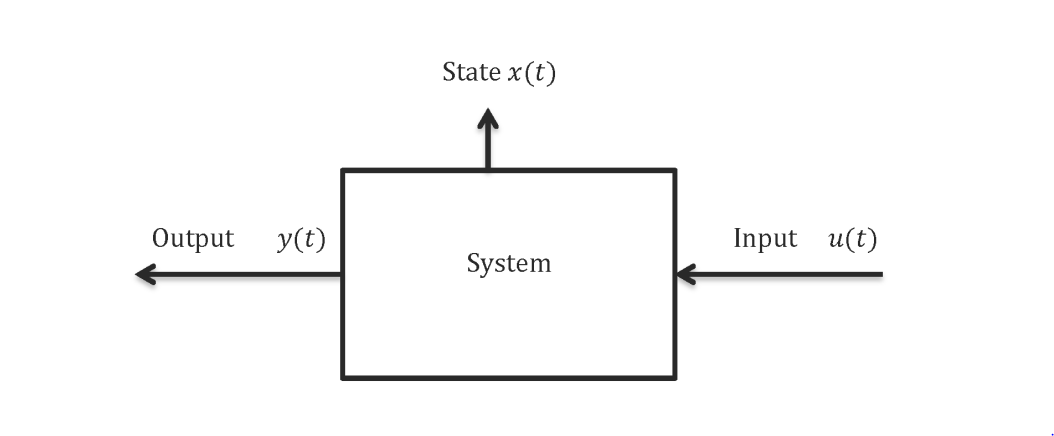
\includegraphics[width=13cm]{Anh1}
  \caption{Sơ đồ khối mô hình không-thời gian liên tục.}
  \label{fig:pic1}
\end{figure}
\begin{example}
Để minh họa rõ hơn việc lập công thức không gian trạng thái, ta xét hệ 2 vật nặng được nối với nhau bởi một lò xo và giảm chấn. Lực $\emph{u}$ tác động vào vật $M_1$, làm thay đổi vị trí $\emph{z}$ của vật $M_2$. Đầu vào của hệ này là lực tác động, đầu ra chính là vị trí của vật $M_2$. Ở đây thứ ta cần quan tâm chính là việc ta có thể điều khiển được vị trí của $M_2$.\\
Áp dụng định luật II Newton, ta có:
\begin{align}
    M_1\ddot{w} &= -b(\dot{w} - \dot{z}) - k(w - z) + u, \\
    M_2\ddot{z} &= b(\dot{w} - \dot{z}) + k(w - z).
\end{align}

\begin{figure}[htp]
\centering
  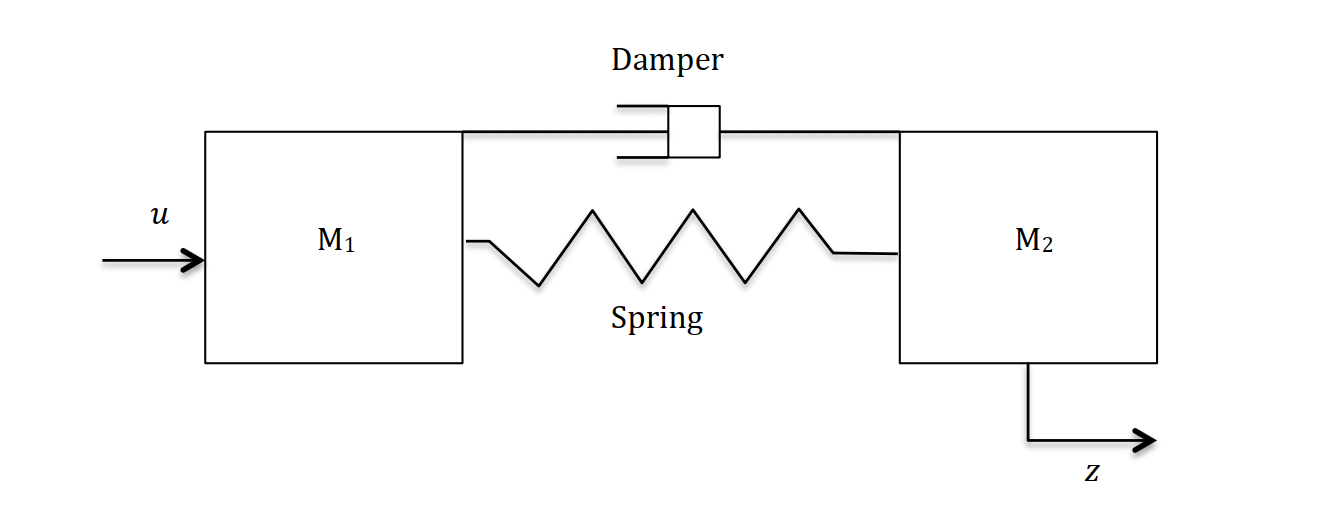
\includegraphics[width=13cm]{Anh2}
  \caption{Hệ vật lò xo giảm chấn.}
  \label{fig:pic2}
\end{figure}

Ở đây, b là hệ số tắt dần, w và z liên tục là sự dịch chuyển  $M_1$ và $M_2$, k là độ cứng của lò xo. Ta đưa hệ đạo hàm bậc 2 này về bậc 1 bằng cách:\\
Đặt $x_1$ = w, $\dot{x_1}$ = $\dot{w}$ = $x_2$, $x_3$ = z, $\dot{x_3}$ = $\dot{z}$ = $x_4$. Khi đó,
\begin{align}
\dot{x}_2 &= -\frac{b}{m_1}(x_2 - x_4) - \frac{k}{m_1}(x_1 - x_3) + u \label{ct2.1.4},  \\
\dot{x}_4 &= \frac{b}{m_2}(x_2 - x_4) + \frac{k}{m_1}(x_1 - x_3) + u, \\
y &= x_3.\label{ct2.1.6}
\end{align}
Ta viết lại \eqref{ct2.1.4}-\eqref{ct2.1.6} hệ dưới dạng ma trận
\begin{align}
    \begin{bmatrix}
        \dot{x}_1\\ \dot{x}_2\\ \dot{x}_3\\ \dot{x}_4
    \end{bmatrix}
     &= 
    \begin{bmatrix}
     0 & 1 & 0 & 0\\
     -\frac{k}{m_1} & -\frac{b}{m_1} & \frac{k}{m_1} & \frac{b}{m_1}\\
     0 & 0 & 0 & 1\\
     \frac{k}{m_2} & \frac{b}{m_2} & -\frac{k}{m_2} & -\frac{b}{m_2}
     \end{bmatrix}
     \cdot
     \begin{bmatrix}
     x_1 \\ x_2 \\ x_3 \\ x_4
     \end{bmatrix}
     + 
     \begin{bmatrix}
     0 \\ \frac{1}{m_1} \\ 0 \\ 0
     \end{bmatrix}
     \cdot u,\\
     y &= 
     \begin{bmatrix}
     0 & 0 & 1 & 0 
     \end{bmatrix}
     \cdot
     \begin{bmatrix}
     x_1 \\ x_2 \\ x_3 \\ x_4
     \end{bmatrix}.
\end{align}
Ta đưa hệ lò xo-giảm chấn này về dạng \eqref{ct2.1.1}
\bigskip
ta có
\newline
A = $\begin{bmatrix}
     0 & 1 & 0 & 0\\
     -\frac{k}{m_1} & -\frac{b}{m_1} & \frac{k}{m_1} & \frac{b}{m_1}\\
     0 & 0 & 0 & 1\\
     \frac{k}{m_2} & \frac{b}{m_2} & -\frac{k}{m_2} & -\frac{b}{m_2}
     \end{bmatrix}
\quad B = \begin{bmatrix}
     0 \\ \frac{1}{m_1} \\ 0 \\ 0
     \end{bmatrix}
\quad C = \begin{bmatrix}
     0 & 0 & 1 & 0 
     \end{bmatrix}
\quad D = 0.$
\end{example}

\section{Nghiệm không gian trạng thái}
Nếu ta đã biết vector \emph{u}, hệ \eqref{ct2.1.1} có thể giải được. Trước khi đi vào cụ thể, ta cần biết một vài định nghĩa \cite{5}.
\begin{definition}
Cho ma trận A cỡ n $\times$ n, khi đó ta định nghĩa \textbf{hàm mũ ma trận} là \[ e^{At} = \sum_{k = 0}^{\infty} \frac{(At)^k}{k!} .\]
\end{definition}
Hai điều lưu ý về hàm mũ ma trận:\\
1. \emph{$e^{A0} = A^0 = I$}. \\
2. \emph{$\frac{d}{dt}e^{At} = \sum_{k = 0}^{\infty} \frac{d}{dt} \frac{A^k t^k}{k!} = \sum_{k = 1}^{\infty} \frac{A^k t^{k-1}}{(k-1)!} = \sum_{k = 0}^{\infty}A\frac{A^k t^k}{k!} = Ae^{At}$}.\\
Ta biết nghiệm của bài toán giá trị ban đầu
\begin{align}
    \dot{x}(t) = Ax(t),\; x(t_0) = x_0, 
\end{align}
là x(t) = $e^{A(t-t_0)}x_0$.\\
Trở lại với phương trình tổng quát với u cho trước,
\begin{align}
    \dot{x}(t) &= Ax(t) + Bu(t), \; x(t_0) = x_0 \label{ct2.2.2} \\ 
    y(t) &= Cx(t) + Du(t). \label{ct2.2.3}
\end{align}
ta sẽ tìm nghiệm qua biến đổi Laplace.
\begin{definition}[Biến đổi Laplace]
Hàm f(x), x $\in$ [0,$\infty$) có biến đổi Laplace là tích phân $\mathcal{L}(f(x))(s)$ = $\hat{f}$(s) = $\displaystyle \int_1^\infty f(x)e^{-sx}dx$ với giá trị s $\in$ $\mathbb{C}$ mà tích phân có nghĩa.
\end{definition}
Hàm Laplace ngược của $\hat{f}$, ký hiệu bởi $\mathcal{L}^{-1} \hat{f}$ = f, là hàm f sao cho biến đổi Laplace của hàm đó chính bằng $\hat{f}$.\\
Để có thể tìm được nghiệm cho hệ phương trình \eqref{ct2.2.2} - \eqref{ct2.2.3}, ta biến đổi Laplace phương trình \eqref{ct2.2.2} và tìm nghiệm $\hat{x}$, cho ta kết quả là
\begin{align}
    \hat{x}(s) = (sI - A)^{-1} x_0 + (sI - A)^{-1} B \hat{u}(s). \label{ct2.2.4}
\end{align}
Áp dụng hàm Laplace ngược \eqref{ct2.2.4} cho ta nghiệm
\begin{align}
    x(t) &= L^{-1}((sI - A)^{-1} x_0) + L^{-1}((sI - A)^{-1} B \hat{u}(t)) \nonumber\\
         &= e^{A(t-t_0)}{x_0} + \displaystyle \int_{t_0}^t e^{A(t-s)}Bu(s)ds. \label{ct2.2.5}
\end{align}
Ta thay phương trình \eqref{ct2.2.5} vào phương trình \eqref{ct2.2.3} ta tìm được $y(t) = Ce^{A(t-t_0)}x_0 + \int_{t_0}^t Ce^{A(t-s)}Bu(s)ds + Du(t).$
\begin{definition}
Ma trận $e^{A(t-t_0)}$ được gọi là \textbf{ma trận chuyển trạng thái}.
\end{definition}
Nếu ta không biết hàm $\emph{u}$, ta có nhiều phương án điều khiển khác nhau để tìm ra hệ điều khiển có thể cho ra đầu ra mong muốn.

\section{Hàm truyền}
Hàm truyền sẽ cho ta thấy mối quan hệ giữa đầu vào và đầu ra của hệ thống và sự ảnh hưởng của nhiễu đối với đầu ra như thế nào.
Để tìm ra hàm chuyển của hệ \eqref{ct2.1.1}
\begin{align}
    \dot{x}(t) &= Ax(t) + Bu(t), \; x(0) = x_0 \label{ct2.3.1} \\ 
    y(t) &= Cx(t) + Du(t) \nonumber
\end{align}
ta sử dụng biến đổi Laplace như \eqref{ct2.2.4} để thu được nghiệm
\begin{align}
    \hat{x}(s) &= (sI - A)^{-1} x_0 + (sI - A)^{-1} B \hat{u}(s), \label{ct2.3.2}\\
    \hat{y}(s) &= C\hat{x}(s) + D\hat{u}(s). \label{ct2.3.3}
\end{align}
Trừ vế theo vế phương trình \eqref{ct2.3.2} cho phương trình \eqref{ct2.3.3} và đặt G(s) = $\frac{\hat{y}(s)}{\hat{u}(s)}$. Phương trình \eqref{ct2.3.3} trở thành 
\begin{align}
    \hat{y}(s) = G(s)\hat{u}(s), \nonumber
\end{align}
hay 
\begin{align}
    G(s) = \frac{\hat{y}(s)}{\hat{u}(s)}.
\end{align}
Hàm G(s) phản ánh tỷ số giữa đầu ra hệ thống $\hat{y}$(s) và đầu vào hệ thống $\hat{u}(s)$ và được gọi là hàm truyền ma trận hoặc đơn giản chỉ là ma trận truyền. Thành phần $G_{ij}$ trong ma trận biểu diễn hàm truyền từ đầu vào thứ j sang đầu ra thứ i. Hàm truyền này đại diện cho các thuộc tính của hệ thống và không đại diện cho độ lớn hoặc tính chất của các đầu vào. Nó cũng không phục vụ cho việc cung cấp bất kỳ thông tin nào về cấu trúc của hệ thống.\\
Một ưu điểm chính của việc sử dụng hàm truyền là chúng cho phép ta làm việc với một hệ thống phức tạp trong miền thời gian và biểu diễn nó như một hàm của một biến trong miền tần số. Thật không may, cách tiếp cận này chỉ hoạt động đối với các hệ thống đơn đầu ra - đơn đầu vào (SISO). Điều này có nghĩa là, đối với nhiều hệ thống đa đầu vào - đa đầu ra, thì sẽ có nhiều hàm truyền được sử dụng để biểu diễn mỗi quan hệ đầu vào - đầu ra. Cần lưu ý rằng, nhiều hệ thống có thể chia sẻ cùng một hàm truyền, không liên quan đến độ lớn của hệ thống hoặc tính chất của đầu vào.
\begin{definition}
Các điểm p mà tại đó hàm truyền G(p) = $\infty$ được gọi là các cực của hệ.
\end{definition}
Nếu G($\infty$) là một ma trận hằng thì hàm truyền được gọi là \textbf{chính} và nếu G($\infty$) = 0, hàm truyền được gọi là \textbf{chính ngặt}.
Chúng ta hãy sử dụng hệ thống giảm chấn khối lượng lò xo từ Ví dụ \eqref{ct2.1.1} để minh họa cách tìm hàm truyền của một hệ đã cho được mô tả bằng biểu diễn không gian trạng thái.
\begin{example}
Từ Ví dụ \eqref{ct2.1.1} ta có
\begin{math}
A = \begin{bmatrix}
     0 & 1 & 0 & 0\\
     -\frac{k}{m_1} & -\frac{b}{m_1} & \frac{k}{m_1} & \frac{b}{m_1}\\
     0 & 0 & 0 & 1\\
     \frac{k}{m_2} & \frac{b}{m_2} & -\frac{k}{m_2} & -\frac{b}{m_2}
     \end{bmatrix},
\quad B = \begin{bmatrix}
     0 \\ \frac{1}{m_1} \\ 0 \\ 0
     \end{bmatrix},\\
     C = \begin{bmatrix}
     0 & 0 & 1 & 0 
     \end{bmatrix},
\quad D = 0.
\\
\\
\\
Suy \; ra \\
G(s) = C(sI - A)^{-1}B + D = \begin{bmatrix}
0 & 0 & 1 & 0
\end{bmatrix}
\begin{pmatrix}
\begin{bmatrix}
s & 0 & 0 & 0 \\
0 & s & 0 & 0 \\
0 & 0 & s & 0 \\
0 & 0 & 0 & s.
\end{bmatrix}
- 
\begin{bmatrix}
0 & 1 & 0 & 0\\
-4 & -2 & 4 & 2\\
0 & 0 & 0 & 1\\
4 & 2 & -4 & -2
\end{bmatrix}
\end{pmatrix}^{-1}
\begin{bmatrix}
0\\
1\\
0\\
0
\end{bmatrix}.
\end{math}
\end{example}
Giản ước đi ta tìm ra 
\begin{align}
    G(s) = \frac{s + 2}{s^4 + 3s^3 + 6s^2}.\nonumber
\end{align}
\begin{definition}
Trong không gian thời gian - trạng thái biểu diễn ở \eqref{ct2.3.1}, ma trận
\begin{align}
    G(iw) = C(iwI - A)^{-1}B + D
\end{align}
được gọi là \textbf{ma trận phản hồi tần số}, $\omega \in \mathbb{R}$ chính \textbf{tần số}.
\end{definition}

\section{Tính điều khiển được và tính quan sát được}
Tính điều khiển và tính quan sát được là những khái niệm cơ bản của lý thuyết điều khiển. Để trình bày những khái niệm này, ta tham khảo trong mục \cite{5}
\begin{definition}
Hệ \eqref{ct2.1.1} 
\begin{align*}
    \dot{x}(t) &= Ax(t) + Bu(t),\\
    y(t) &= Cx(t) + Du(t)
\end{align*}
được gọi là có thể điều khiển được nếu hệ thống đạt được bất kì trạng thái bất kì $x_1 = x(t_1)$, trong thời gian hữu hạn $t_1$, từ bất kỳ trạng thái ban đầu x(0) bằng cách chọn điều khiển u(t), $0 \leq t \leq t_1$ phù hợp.
\end{definition}
Tính điều khiển của hệ thống \eqref{ct2.1.1}, được gọi là tính điều khiển của cặp (A, B). Định lý sau cung cấp các điều kiện có thể kiểm chứng được về việc một hệ thống có thể điều khiển được hay không.
\begin{theorem}\label{dly2.4.1}
Cho A  $\in \mathbb{R}^{n\times n}$  và  B  $\in \mathbb{R}^{n\times m}(m \leq n).$ Các điều sau đây là tương đương:
 \renewcommand{\theenumiii}{\roman{enumii}}
 \begin{enumerate}
    \item Hệ \eqref{ct2.1.1} có thể điều khiển được.
    \item Ma trận điều khiển $n \times nm$ là $C_M$ = $[B, AB, A^2B,...,A^{n-1}B]$ có đủ hạng dòng.
    \item Ma trận
    \begin{align*}
        W_C = \int_{0}^{t_1}e^{At}BB^{T}e^{A^{T}t}dt
    \end{align*}
không suy biến với bất kỳ $t_1$ > 0.
    \item Nếu ($\lambda$, x) là một cặp giá trị riêng và vector riêng tương ứng của $A^{T}$, thì $x^{T}B \ne$ 0.
    \item Rank(A - $\lambda$ I, B) = n với mọi giá trị riêng $\lambda$ của A.
    \item Các giá trị riêng của A - BK có thể được phân bố tùy ý bằng một lựa chọn thích hợp của K.
 \end{enumerate}
\end{theorem}
\newpage
\begin{definition}
Hệ thời gian liên tục \eqref{ct2.1.1} gọi là $\textbf{quan sát được}$ nếu tồn tại $t_1$> 0 sao cho trạng thái ban đầu x($t_0$) xác định duy nhất nếu biết u(t) và y(t) với mọi $0 \leq t \leq  t_1 $. 
\end{definition}
Tính quan sát được của hệ thống \eqref{ct2.1.1} được gọi là tính quan sát được của cặp (A, C).Tính đối ngẫu có nghĩa là cặp (A, C) có thể quan sát được nếu cặp ($A^{T}, C^{T}$) có thể điều khiển được. Do tính hai mặt của khả năng quan sát và khả năng điều khiển, khả năng quan sát có các đặc điểm tương tự như tính điều khiển được trong Định lý 2.4.1.
\begin{theorem}
Những điều sau đây là tương đương:
\renewcommand{\theenumiii}{\roman{enumii}}
\begin{enumerate}
    \item Hệ \eqref{ct2.1.1} có thể quan sát được.
    \item Ma trận của khả năng quan sát $O_M$ = $[C CA ... CA^{n-1} ]^{T}$ có hạng đủ.
    \item Ma trận
    \begin{align*}
        W_O = \int_{0}^{t_0}e^{A^{T}t}C^{T}Ce^{At}dt
    \end{align*}
không suy biến với mọi $t_1$ dương.
    \item Ma trận 
    \begin{math}
        \begin{bmatrix}
    \lambda I -A \\
    C
    \end{bmatrix}
    \end{math}
có hạng bằng n với mọi giá trị riêng của A.
    \item Nếu ($\lambda$, y) là 1 cặp giá trị riêng và vector riêng của A, thì $C_y \neq$ 0.
    \item Các giá trị riêng cho A - LC có thể được gán tùy ý bằng một lựa chọn thích hợp của L.
\end{enumerate}
\end{theorem}
Khả năng điều khiển và khả năng quan sát đóng vai trò quan trọng trong sự tồn tại của các nghiệm xác định dương và nửa xác định dương cho phương trình Lyapunov.
\begin{definition}
Ma trận A được gọi là \textbf{ma trận ổn định} nếu mọi giá trị riêng của A có phần thực âm thực sự.
\end{definition}
\begin{definition}
Cho A là một ma trận ổn định, thì 
\begin{align}
    C_G = \int_{0}^{t_1}e^{At}BB^{T}e^{A^{T}t}dt
\end{align}
gọi là \textbf{Grammian điều khiển.}
\end{definition}
\begin{definition}
Cho A là một ma trận ổn định, thì
\begin{align}
    O_G = \int_{0}^{\infty}e^{A^{T}t}C^{T}Ce^{At}dt 
\end{align}
được gọi là \textbf{Grammian quan sát.}
\end{definition}
\begin{theorem}\label{dly2.4.3}
Cho A là một ma trận ổn định. Grammian điều khiển $C_G$ thỏa mãn phương trình Lyapunov
\begin{align}
    AC_G + C_GA^{T} = -BB^{T}
\end{align}
và là đối xứng, xác định dương khi và chỉ khi (A, B) có thể điều khiển được.
\end{theorem}
\begin{theorem}\label{dly2.4.4}
Cho A là 1 ma trận ổn định. Grammian quan sát $O_G$ thỏa mãn phương trình Lyapunov
\begin{align}
    O_GA + A^{T}O_G = -C^{T}C
\end{align}
và là đối xứng, xác định dương khi và chỉ khi (A, B) có thể quan sát được.
\end{theorem}
Sau đây là một ví dụ minh họa tính toán của cả 2 giá trị $C_G$ và $O_G$.
\begin{example}
Trở lại hệ \eqref{ct2.1.1}, với 
\begin{align*}
    A = \begin{bmatrix}
        -4 & -8 & -12\\
        0 & -8 & -4\\
        0 & 0 & 0
    \end{bmatrix}, \; B = \begin{bmatrix}
        1\\
        1\\
        1
    \end{bmatrix}, \;  C = [1 \quad 1 \quad 1], \; D = 0.
\end{align*}
Ma trận A ổn định và sử dụng lệnh \textbf{lyap} trong  MATLAB để giải các phương trình Lyapunov trong Định lý 1.4.5 và 1.4.6, chúng ta tìm được
\begin{align*}
    C_G = \begin{bmatrix}
        0.1458 & 0.0208 & 0.0208\\
        0.0208 & 0.0833 & 0.0833\\
        0.0208 & 0.0833 & 0.0833
    \end{bmatrix} = O_G.
\end{align*}
Ta nhận thấy ma trận này có hai dòng bằng nhau nên định thức ma trận bằng 0, suy ra ma trận suy biến, nên (A, B) không điều khiển được và (C, D) không quan sát được.
\end{example}

\section{Tính ổn định hóa được và khả năng phát hiện được}
Một bộ điều khiển thường được thiết kế để ổn định hóa một hệ thống tuyến tính. Điều này được thực hiện bằng cách chọn một điều khiển $u$ thích hợp sao cho ma trận hệ đóng kín $(A - BK)$ ổn định, trong đó $K$ là ma trận phản hồi mà $u(t) = Kx(t)$. Trong phần này, chúng ta xác định tính ổn định hóa được của một hệ thống và trình bày các đặc điểm của hệ thống có thể được ổn định hóa được thông qua điều khiển phản hồi.\\
Đầu tiên chúng ta chọn hệ chưa điều khiển
\begin{align}\label{ct2.5.1}
    \dot{x}(t) = Ax(t), \quad x(0) = x_0.
\end{align}
\begin{definition}
Trạng thái cân bằng của hệ \eqref{ct2.5.1}, là vectơ $x_e$ thỏa mãn
\begin{align}
    Ax_e = 0.
\end{align}
Nếu ma trận A không suy biến, phương trình trên chỉ có nghiệm tầm thường $x_e$ = 0.
\end{definition}
\begin{definition}
Gọi $x_e$ là trạng thái cân bằng của \eqref{ct2.5.1}, thì $x_e$ được gọi là
\begin{enumerate}
    \item ổn định nếu với mỗi $\epsilon$ > 0 tồn tại $\delta$ > 0  sao cho $\norm{x(t) - x_e}$ < $\epsilon$,  $\forall$ t $\geq$ 0 nếu $\norm{x(t_0) - x_e} < \delta$.
    \item ổn định tiệm cận nếu trạng thái cân bằng ổn định và $\exists \delta > 0$ sao cho $\norm{x(t_0) - x_e} < 0$ dẫn đến $\displaystyle \lim_{x\to\infty} x(t) = x_e$.
\end{enumerate}
\end{definition}
Điều này có nghĩa là mọi nghiệm đúng của hệ nếu bắt đầu đủ gần điểm cân bằng ổn định tiệm cận, thì sẽ tiến gần đến điểm cân bằng khi thời gian tăng. Nên nếu $x_e = 0$ và \emph{A} không suy biến, hệ không ổn định được ở trên ổn định tiệm cận nếu $\emph{x(t)} \to 0 \; khi \; \emph{t} \to \infty.$
Các giá trị riêng của ma trận A trong \eqref{ct2.5.1} đặc trưng cho độ ổn định của hệ thống.
\begin{theorem}
Hệ thống \eqref{ct2.5.1} ổn định tiệm cận khi và chỉ khi mọi giá trị riêng của A có phần thực âm thực sự.
\end{theorem}
Cũng như với tính điều khiển, nghiệm của phương trình Lyapunov cũng đặc trưng cho tính ổn định của \eqref{ct2.5.1}.
\begin{theorem}
Hệ:
\begin{align*}
    \dot{x}(t) = Ax(t)
\end{align*}
ổn định tiệm cận khi và chỉ khi với ma trận M đối xứng dương bất kỳ, thì phương trình sau có nghiệm duy nhất
\begin{align*}
    XA + A^{T}X = -M.
\end{align*}
\end{theorem}
Xét hệ tuyến tính \eqref{ct2.1.1},
\begin{align*}
    \dot{x}(t) &= Ax(t) + Bu(t),\\
    y(t) &= Cx(t) + Du(t).
\end{align*}
Ta xét việc tìm nghiệm điều khiển \emph{u} để đưa hệ sang một trạng thái mong muốn. Điều đó có nghĩa là tìm 1 \textbf{ma trận phản hồi} $K$ sao cho $A - BK$ ổn định. Không phải mọi hệ có thể đưa về một trạng thái nhất định, nên điều quan trọng nhất của phần này là tìm ra điều kiện cần và đủ sao cho tồn tại một ma trận phản hồi ổn định.\\
Hơn nữa giả sử ta có thể tìm được mọi thông tin của trạng thái \emph{x(t)} ở mọi thời gian \emph{t} bất kỳ. Sử dụng điều khiển tuyến tính, ta suy ra 
\begin{align}
    u(t) = -Kx(t).
\end{align}
Trừ vế theo vế phương trình \emph{u(t) = -Kx(t)} cho phương trình \eqref{ct2.1.1} ta được \textbf{hệ kín}:
\begin{align}\label{ct2.5.4}
    \dot{x}(t) &= (A - BK)x(t),\\
    y(t) &= (C - DK)x(t).
\end{align}
Ta nhắc lại hệ không điều khiển được \eqref{ct2.5.1}
 ổn định khi ma trận A ổn định. Vậy nên việc ổn định hóa hệ \eqref{ct2.5.4} quy về việc tìm ma trận  $K$ sao cho $(A - BK)$ là ổn định. Nếu tồn tại một ma trận $K$, thì $K$ được gọi là \textbf{ma trận phản hồi} và ổn định hóa được, cặp ma trận (A, B) được gọi là \textbf{cặp ma trận ổn định hóa được}.\\
 Những định lý sau đây cho ta điều kiện cần và đủ để đánh giá việc có thể ổn định được ma trận cho 1 hệ đang xét.\\
 \begin{theorem}
  Những khẳng định sau là tương đương:
 \begin{enumerate}
     \item Cặp ma trận (A, B) là ổn định hóa được.
     \item Rank(A - $\lambda I$, B) = n, với mọi Re($\lambda$) $\geq$ 0.
     \item Với mọi $\lambda$ và x $\ne$ 0, nếu $x^{*}$A = $\lambda x^{*}$ và Re($\lambda$) $\geq$ 0 thì $x^{*}B \ne$ 0.
 \end{enumerate}
 \end{theorem}
 \begin{coroll}
 Nếu cặp (A, B) là điều khiển được,  thì nó cũng ổn định hóa được.
 \end{coroll}
 Lưu ý khả năng điều khiển suy ra khả năng ổn định chỉ là chiều suy ra mà không suy ngược lại.\\
 Cũng như khả năng quan sát được đối ngẫu với khả năng điều khiển được, khả năng ổn định được của hệ thống cũng đối ngẫu với khả năng phát hiện được.\\
 \begin{definition}
 Hệ được gọi là \textbf{phát hiện được} nếu tồn tại ma trận L sao cho với cặp ma trận (A, C) thì A - LC là ổn định.
 \end{definition}
\begin{theorem}
Các điều sau đây là tương đương:
\begin{enumerate}
    \item Cặp ma trận (A, C) là phát hiện được.
    \item Ma trận 
    $\begin{bmatrix}
        \lambda I - A \\
        C.
    \end{bmatrix}$
    có hạng đầy đủ, với mọi $Re(\lambda) \geq$ 0.
    \item Với mọi $\lambda$ và x $\ne$ 0 sao cho Ax = $\lambda$x và Re($\lambda) \geq$ 0, thì Cx $\ne$ 0.
    \item Cặp ma trận ($A^{T}$, $C^{T}$) là ổn định hóa được.
\end{enumerate}
\end{theorem}
Có thể thấy rằng một hệ thống có thể điều khiển được thì các giá trị riêng của hệ điều khiển đóng kín có thể được gán tùy ý (bài toán gán giá trị riêng). Vấn đề với việc chỉ định các giá trị riêng tùy ý đó là không có phương pháp luận để tìm một bộ điều khiển tối ưu sao cho các đặc điểm thiết kế hệ thống có thể đáp ứng một cách hiệu quả nhất có thể.\\
Điều này dẫn đến nhiều phương pháp điều khiển tối ưu ví dụ như điều khiển tối ưu tuyến tính bậc hai. Phương pháp này tối thiểu hóa hàm phạt bậc 2 đã được xác định trước. Tuy nhiên, lưu ý \cite{7} cho ta sự phát triển song song của điều khiển \hinf và điều khiển \emph{$H_2$} tối ưu hay còn được gọi là điều khiển dạng toàn phương tuyến tính Gauss.

\section{Chuẩn \hinf}
Trước tiên, hãy lưu ý rằng hàm truyền của một hệ thống ổn định bất kỳ được mô hình hóa bởi phương trình vi phân tuyến tính hệ số hằng là hàm hữu tỉ và có các cực nằm hoàn toàn trong nửa mặt phẳng bên trái và là giải tích trong nửa mặt phẳng bên phải. Một không gian của các hàm như vậy được gọi là không gian Hardy, ký hiệu là \hinf. Đối với hệ đa biến bất kỳ, hàm truyền G(i$\omega$) là một ma trận. Các giá trị kỳ dị của ma trận A, $\sigma_j$(A) được định nghĩa là
\begin{align*}
    \sigma_j(A) = \sqrt{\lambda_j(AA^{T})},
\end{align*}
trong đó $\lambda_j$(E) là giá trị riêng thứ j của ma trận E.
\newline
\newline
Chuẩn Euclid của ma trận là:
\begin{align*}
    \norm{A} = \displaystyle \max_{i}\sigma_i(A).
\end{align*}
Suy ra
\begin{align*}
    \norm{G(i\omega)} = \displaystyle \max_{i}\sigma_i(G(i\omega)) = \sigma_{max}(G(i\omega)).
\end{align*}
\begin{definition}
Chuẩn \hinf của hàm truyền G(s) được định nghĩa là
\begin{align}
    \norm{G}_{\infty} = \sup_{\omega \in \mathbb{R}}\sigma_{max}(G(i\omega)).
\end{align}
\end{definition}
\smallskip
Chuẩn này cung cấp một cách khác để phân tích tính ổn định của hệ thống, cụ thể là nếu G(s) $\in$ \hinf thì hệ thống ổn định. Như được mô tả trong \cite{15} cho trường hợp khi G là hữu tỉ, G $\in$ \hinf khi và chỉ khi G không có cực trong nửa mặt phẳng đóng bên phải.
\newpage

\chapter{Thuật toán: Miền tần số}
\chapter{Một số trường hợp đặc biệt trong phân tích tính chất ổn định của các hệ động lực có trễ}
\setlength{\parindent}{6.5ex}

\section{Giới thiệu}
Ta xét hệ điều khiển có trễ với hệ số hằng được biểu diễn bằng phương trình vi phân có trễ dạng
\begin{equation}\label{eq1}
	\dot{x}(t)=Ax(t) + Bx(t -\tau). 
\end{equation}
%Phân tích tính ổn định và điều khiển của hệ thống này là một lĩnh vực nghiên cứu rộng lớn. Khó khăn của các hệ này nảy sinh từ thực tế là độ trễ $\tau$ làm cho hệ \eqref{eq1} là vô hạn chiều. Một tổng hợp tốt về những kết quả gần đây và những thách thức trong lĩnh vực này có thể tìm được trong \cite{Sip11} (2011). Việc nghiên cứu tính ổn định và tính điều khiển được của loại hệ thống này đã được nhiều nhà toán học quan tâm. Một số công trình nghiên cứu các miền ổn định tuyệt đối liên quan đến thời gian trễ (Olgac \& Sipahi, 2002; Sipahi \& Olgac, 2006), và dẫn đến thời gian trễ được sử dụng như một công cụ điều khiển tính ổn định (Olgac, Ergenc, \& Sipahi, 2005). Các nghiên cứu khác tập trung vào việc tính toán các giá trị riêng của hệ thống. Các công trình này bao gồm các phương pháp tiếp cận dựa trên việc rời rạc hóa các nghiệm  (Breda, 2006 ; Butcher \& Bobrenkov, 2011 ; Engelborghs, Luzyanina và Roose, 2002) hoặc toán tử sinh \cite{Bre09}, và phương pháp này dựa trên việc tìm nghiệm của phương trình đặc trưng \cite{Vyh09}. Từ đây các phương pháp đã được đề xuất để tối ưu hóa việc tính toán các giá trị riêng trội.  (Michiels, Engelborghs, Vansevenant, \& Roose, 2002; Mondié \& Michiels, 2003). Cuối cùng phương pháp Krylov để tính các giá trị riêng cho các bài toán có cỡ lớn  đã được đề xuất trong (Michiels, Engelborghs, Vansevenant, \& Roose, 2002; Mondié \& Michiels, 2003).  \\
%Trong thập kỉ trước, một công trình để phân tích DDEs dựa trên hàm Lambert W đã được phát triển (\cite{AslU03}; Yi, 2009; \cite{Yi10}). Nó mở rộng công trình trước đó của Wright( 1959). Ý tưởng chính của phương pháp này là biểu diễn nghiệm của một phương trình vi phân có trễ dưới dạng tổng của một chuỗi vô hạn các hàm mũ. Giá trị riêng của hệ được tìm ra bằng việc sử sụng hàm Lambert W. Vì bài toán là sự vô hạn chiều, ta  giả sử rằng có một tương ứng 1 - 1 giữa các giá trị riêng của hệ với các nhánh của hàm. 
%
Như trong chương trước chúng ta đã thấy việc phân tích tính chất ổn định của hệ đã được giải quyết bằng việc sử dụng các giá trị riêng trội của hệ tương ứng với các nhánh thứ 
$k = 0, \pm 1 , \cdots , \pm m$, trong đó $m$ là số khuyết của ma trận $B$ (tức là số chiều của hạt nhân ma trận) trong \eqref{eq1}. Do đó, chỉ có một số nhánh hữu hạn được xem xét để xác định xem một nghiệm có ổn định hay không, hoặc để đánh giá tốc độ tăng/giảm của nghiệm. 
%Hơn nữa, sự tồn tại công thức nghiệm hiển của hệ biểu diễn dưới dạng chuỗi lũy thừa cho phép phân tích các đặc tính cấu trúc cũng như tính quan sát được và tính điều khiển được của các hệ DDE \cite{Yi08}, sự phát triển của các kỹ thuật đặt cực để tổng hợp điều khiển (\cite{YiEig10}, \cite{YiMay10};\cite{YiJune12}; \cite{YiDes10}) và các ứng dụng khác như ước lượng tốc độ phân rã \cite{Du12} và thiết kế phổ ( Wei, Bachrathy, Orosz, \& Ulsoy, 2014).\\
Nền tảng cơ bản của phương pháp luận này là giả thiết rằng nhánh chính của hàm Lambert W xác định sự ổn định của hệ thống. Điều này đã được chứng minh cho các hệ thống bậc nhất (\cite{AslU03}; \cite{Shi06}). Tuy nhiên với trường hợp bậc cao hơn, kết quả này không được mở rộng chặt chẽ, và chỉ dựa trên các quan sát của Yi, Nelson và Ulsoy trong \cite{Yi07}.

%Điều này không mâu thuẫn với giả thuyết liên quan đến sự ổn định nhưng góp phần bổ sung thêm cho hiểu biết về phổ của hệ nhiều chiều có trễ.
 
Trong chương này, ta chỉ ra rằng giả thiết trên nói chung không hoàn toàn đúng. Bằng việc nghiên cứu các hệ bậc hai cụ thể với cấu trúc rấ phổ biến trong các ứng dụng, ta chỉ ra rằng toàn bộ phổ của hệ thống \eqref{eq1} có thể tìm được mà chỉ cần sử dụng hai nhánh của hàm Lambert W (thay vì $2m+1$ nhánh như trong Giả thiết \ref{Hypo}), tức là không có tương ứng một - một nào giữa các giá trị riêng và các nhánh của hàm Lambert W. Điều này do thực tế rằng một phương trình phi tuyến quan trọng trong cách tiếp cận sử dụng hàm Lambert không có nghiệm duy nhất. Hơn nữa, ta chỉ ra rằng nhánh chính không những có thể sử dụng để tìm nghiệm trội nhất của hệ mà còn có thể dùng để tìm các nghiệm khác nữa. \ Cấu trúc của chương này như sau. Mục \ref{sec4} trình bày về hệ bậc hai và những kết quả chính thu được khi phân tích hệ đó. Những phân tích này được minh họa bằng thử nghiệm số trong mục 5. Mục 6, ta sẽ trình bày các thảo luận trong một trường hợp đặc biệt khác mà kết quả của mục 4 không thể áp dụng trực tiếp. Cuối cùng, ta đưa ra một số kết luận của nghiên cứu trong mục 7.\\


\section{Một trường hợp đặc biệt của hệ bậc hai}\label{sec4}
Xét hệ \eqref{eq9}, với $A$ và $B$ là các ma trận có dạng sau
\begin{equation}\label{eq16}
	A= \begin{bmatrix}
		0 &1\\
		a_{21} &a_{22}
	\end{bmatrix}, \quad
	B= \begin{bmatrix}
		0 &0\\
		b_{21} &b_{22}
	\end{bmatrix}.
\end{equation}
Từ \eqref{eq16}, ta có hạng của $B$ bằng $1$, lí thuyết dự đoán rằng nghiệm của \eqref{eq14} tương ứng với $k =0$ và $k = \pm1$ cho ta các nghiệm trội của bài toán. \\
Từ cấu trúc của $B$, ta thấy $M_k = \tau B Q_k$ có dạng
\begin{equation}\label{eq17}
	M_k = \begin{bmatrix}
		0 &0\\
		m_{21} &m_{22}
	\end{bmatrix}.
\end{equation}
Theo định nghĩa của ma trận hàm Lambert W, sử dụng trường hợp nhánh chuyển mạch, vì $M_k$ có một giá trị riêng bằng $0$.\\
Nếu $m_{22} \ne 0$, ta có
\begin{equation}\label{eq18}
	W_k(M_k)= \begin{bmatrix}
		0 &0\\
		\dfrac{	m_{21}}{m_{22}} W_k(m_{22}) &W_k(m_{22})
	\end{bmatrix}.
\end{equation}
Từ đó ta được
\begin{equation}\label{eq19}
	S_k = \dfrac{1}{\tau}W_k(M_k)+A = 
	\m{0 &1\\
		\dfrac{	m_{21}}{\tau m_{22}} W_k(m_{22}) +a_{21} &\dfrac{1}{\tau}W_k(m_{22})+a_{22}}
	 \ .
\end{equation}
Nếu $m_{22}=0, m_{21} \ne 0$, ta được
\begin{equation}\label{eq20}
	S_k	= \begin{bmatrix}
		0 &1\\
		\dfrac{	m_{21}}{\tau} +a_{21} &a_{22}
	\end{bmatrix},
\end{equation}
trong đó, ta sử dụng $W_0 (0)' =1$. Bây giờ, ta sẽ phát biểu kết quả chính của bài toán.\\
%
\noindent\textbf{Định lý 1.} \textit{Cho $A$ và $B$ được cho bởi \eqref{eq16}. Lấy $\{ \lb, \overline{\lb}\}$ là một cặp giá trị riêng liên hợp bất kỳ. Giả sử bội của chúng bằng một. Khi đó, với $k =0$ hoặc $k =-1$, tồn tại một nghiệm thực của \eqref{eq14}, sao cho nếu nghiệm này và giá trị $k$ tương ứng được chọn trong bước đầu tiên của Thuật toán 1 thì giá trị riêng $\lb$ và $\overline{\lb}$ được tìm thấy trong bước cuối cùng của thuật toán. }\\
%
\noindent\textbf{Chứng minh.} Ý tưởng chính là thực hiện các bước của Thuật toán 1 theo thứ tự ngược lại.\\
Ta xây dựng một ma trận thực $S_k$ nhận cặp  $\{ \lb, \overline{\lb}\}$ là giá trị riêng là
\begin{equation}\label{eq21}
	S_k = \begin{bmatrix}
		0 &1\\
		-\vert \lb \vert ^2 & 2 \re(\lb)
	\end{bmatrix}.
\end{equation}
Sau đó, ta xây dựng $M_k$ từ \eqref{eq21}. Xét hai trường hợp sau.\\
\noindent\textit{Trường hợp 1:} $2\re(\lb) \ne a_{22}$.\\
So sánh \eqref{eq19} và \eqref{eq21}, ta lấy $M_k$ có dạng \eqref{eq17}, trong đó $m_{21} \in \R$ và $m_{22} \in \R$ được chọn sao cho thỏa mãn phương trình sau
\begin{equation*}
	\heva{2\re(\lb) = \dfrac{1}{\tau} W_k(m_{22}) +a_{22} \\ -\vert \lb\vert ^2 = \dfrac{m_{21}}{\tau m_{22}} W_k(m_{22}) + a_{21}}.
\end{equation*}
Từ đó suy ra
\begin{equation}\label{eq22}
	W_k(m_{22}) = \tau(2\re(\lb) - a_{22}).
\end{equation}

\begin{equation}\label{eq23}
	m_{21} = -\dfrac{m_{22}(\vert \lb \vert ^2 +a_{21})}{2\re(\lb)-a_{22}}.
\end{equation}
Lựa chọn như vậy luôn thực hiện được với $k = 0$ hoặc $k = -1$. Phương trình \eqref{eq22} ngụ ý rằng $W_k(m_{22})$ phải là một số thực. Như đã đề cập trước đó, theo định nghĩa nhánh cắt của hàm Lambert W thì chỉ có hai nhánh cho giá trị thực là nhánh chính $k = 0$ và nhánh $k = -1$ và hợp hai miền giá trị của $W_0$ và $W_{-1}$ chứa tập số thực $\R$ (xem hình 1). Hơn nữa, trong trường hợp này, $m_{22} \ne 0$, đó là lí do của việc sử dụng \eqref{eq19}.\\
%
\noindent\textit{Trường hợp 2:} $2\re(\lb) = a_{22}$.\\
Ta có $\dfrac{1}{\tau} W_k(m_{22}) = 0$. Do đó $W_k(m_{22}) =0$. Vì vậy $m_{22}=0$.\\
Khi đó
\begin{equation*}
S_k = \begin{bmatrix}
	0 &1\\
	\dfrac{m_{21}}{\tau} +a_{21} & a_{22}
\end{bmatrix}.
\end{equation*}
Vì vậy $m_{21} = - \tau(\vert \lb \vert ^2 + a_{21})$.\\
Do vậy
\begin{equation}\label{eq24}
	M_k = \begin{bmatrix}
		0 &0\\
		- \tau(\vert \lb \vert ^2 + a_{21}) & 0
	\end{bmatrix}
\end{equation} 
Cuối cùng, ta có cặp $(k, M_k)$ được xây dựng như trên là một nghiệm của \eqref{eq14}.\\
Thật vậy, lấy $\mathbf{v}$ và  $\mathbf{\overline{v}}$ là các vector riêng tương ứng với các giá trị riêng $\lb$ và $\overline{\lb}$. Nếu $\lb$ là giá trị riêng có bội bằng $1$, thì cặp $(\mathbf{V}, \mathbf{\lb})$ là một cặp bất biến của \eqref{eq9}, trong đó
\begin{equation}\label{eq25}
	\mathbf{V} := \begin{bmatrix}
		\mathbf{v} &\mathbf{\overline{v}}
	\end{bmatrix},
	\quad 
	\mathbf{\lb} := \mathrm{diag} (\lb, \overline{\lb}).
\end{equation}
Ta có
\begin{align}\label{100}
	&\mathbf{V} \mathbf{\lb} - A - B \mathbf{V} \exp (-\mathbf{\lb})\\ \notag
	&= 
	\begin{bmatrix}
		\mathbf{v}&\mathbf{\overline{v}}
	\end{bmatrix}
	\begin{bmatrix}
		\lb & 0 \\ 0 & \overline{\lb}
	\end{bmatrix}
	- A - B \begin{bmatrix}
		\mathbf{v}&\mathbf{\overline{v}}
	\end{bmatrix} \exp \left(\begin{bmatrix}
		\lb & 0 \\ 0 & \overline{\lb}
	\end{bmatrix}\right)\\ \notag
	&= \begin{bmatrix}
		\mathbf{v}&\mathbf{\overline{v}}
	\end{bmatrix}
	\begin{bmatrix}
		\lb & 0 \\ 0 & \overline{\lb}
	\end{bmatrix}
	- A - B \begin{bmatrix}
		\mathbf{v}&\mathbf{\overline{v}}
	\end{bmatrix} \begin{bmatrix}
		e^{\lb} & 0 \\ 0 & e^{\overline{\lb}}
	\end{bmatrix}.
\end{align} 
Ta có phương trình đặc trưng
\begin{equation*}
	det(\lb I_2 -A - Be^{-\lb \tau}) = 0 .
\end{equation*}
Vì $\mathbf{v}$ và  $\mathbf{\overline{v}}$ là các vector riêng nên ta có
\begin{equation*}
	\heva{
		&(\lb I_2 -A - Be^{-\lb \tau})\mathbf{v} =0\\
		&(\overline{\lb} I_2 -A - Be^{-\overline{\lb} \tau}) \mathbf{\overline{v}} =0} .
\end{equation*}
Từ đó suy ra
\begin{equation*}
	\heva{
		&\lb \mathbf{v} -A\mathbf{v} - Be^{-\lb \tau}\mathbf{v} =0\\
		&\overline{\lb}\mathbf{\overline{v}} -A\mathbf{\overline{v}} - Be^{-\overline{\lb} \tau}\mathbf{\overline{v}} =0} .
\end{equation*}
Như vậy
\begin{equation}\label{200}
	\begin{bmatrix}
		\mathbf{v}&\mathbf{\overline{v}}
	\end{bmatrix}
	\begin{bmatrix}
		\lb & 0 \\ 0 & \overline{\lb}
	\end{bmatrix}
	- A - B \begin{bmatrix}
		\mathbf{v}&\mathbf{\overline{v}}
	\end{bmatrix} \begin{bmatrix}
		e^{\lb\tau} & 0 \\ 0 & e^{\overline{\lb} \tau}
	\end{bmatrix} = \begin{bmatrix}
		0\\0
	\end{bmatrix}.
\end{equation}
Từ \eqref{100} và \eqref{200} ta thấy $\mathbf{V}$ và $\mathbf{\lb}$  thỏa mãn phương trình
\begin{equation}\label{eq26}
	\mathbf{V} \mathbf{\lb} - A - B \mathbf{V} \exp (-\mathbf{\lb})=0.
\end{equation}
Ta có thể kiểm tra trực tiếp $S_k$ có phân tích Jordan là
\begin{equation}\label{eq27}
	S_k = \mathbf{V} \mathbf{\lb} \mathbf{V}^{-1}.
\end{equation}
Từ đó ta có
\begin{equation}\label{eq28}
	\exp(-S_k) = \exp (-\mathbf{V} \mathbf{\lb} \mathbf{V}^{-1}) = \mathbf{V} \exp(-\mathbf{\lb}) \mathbf{V}^{-1}.
\end{equation}
Suy ra
\begin{equation}\label{eq29}
	\mathbf{V} \mathbf{\lb} = S_k \mathbf{V}, \quad \mathbf{V} \exp(-\mathbf{\lb}) = \exp(-S_k) \mathbf{V}.	
\end{equation}
Thay vào \eqref{eq26}, với $V$ khả nghịch, ta được
\begin{equation}\label{eq30}
	S_k -A - B \tau \exp (-S_k \tau) =0 .
\end{equation}
Cuối cùng, thay $S_k$ bởi 
\begin{equation}\label{eq31}
	S_k = \dfrac{1}{\tau}W_k(M_k)+A
\end{equation}
ta được kết quả trong \eqref{eq14}.\\
\noindent\textbf{Định lý 2.} \textit{Cho $A$ và $B$ được cho bởi \eqref{eq16}. Lấy $\lb_1 \ne \lb_2$ là hai giá trị riêng thực bội đơn của phương trình đặc trưng của hệ cho bởi \eqref{eq16}. Sau đó, cho $k =0$ hoặc $k =-1$, tồn tại một nghiệm thực của \eqref{eq14}, sao cho nếu nghiệm này và giá trị $k$ tương ứng được chọn trong bước đầu tiên của thuật toán 1 thì giá trị riêng $\lb_1$ và $\lb_2$ được tìm thấy trong bước cuối cùng của thuật toán. }\\
\noindent\textbf{Chứng minh.} Chứng minh hoàn toàn tương tự với mệnh đề 1. Ta xây dựng ma trận $S_k$ nhận $\lb_1$ và $\lb_2$ làm giá trị riêng là
\begin{equation}\label{eq32}
	S_k =\begin{bmatrix}
		0 & 1\\ 
		- \lb_1 \lb_2 & \lb_1 + \lb_2
	\end{bmatrix}
\end{equation}
Tiếp theo ta sẽ xây dựng ma trận $M_k$. Xét hai trường hợp:\\
\noindent\textit{Trường hợp 1.} $\lb_1 + \lb_2 \ne a_{22}$\\
Ta đi tìm $m_{21}$ và $m_{22}$ sao cho
\begin{equation*}
	\heva{
		&W_k(m_{22}) = \tau (\lb_1 + \lb_2 -a_{22})\\ 
		&m_{21} = - \dfrac{m_{22}(\lb_1 \lb_2+a_{21})}{\lb_1  + \lb_2 - a_{22}}
	} . 
\end{equation*}
Điều này luôn thực hiện được cho trường hợp $k =1$ hoặc $k =0$ và $W_k(M_{22})$ phải là số thực. \\
\noindent\textit{Trường hợp 2.} $\lb_1 + \lb_2 = a_{22}$
\begin{equation*}
	M_k = \begin{bmatrix}
		0 & 0\\
		-\tau (\lb_1 \lb_2 +a_{21}) & 0
	\end{bmatrix}.
\end{equation*}
Ta có cặp $(k, M_k)$ chính là một nghiệm của \eqref{eq14}.\\
Từ Định lý 1 và 2, ta thu được hệ quả sau.\\ 

\noindent\textbf{Hệ quả 1.} \textit{Cho $A$ và $B$ được cho bởi \eqref{eq16}. Nếu tất cả các giá trị riêng của \eqref{eq16} là đơn và  nếu số lượng các giá trị riêng thực khác một, bằng cách lựa chọn ban đầu $M_k$ thích hợp cho phương trình \eqref{14},  thì tất cả các giá trị riêng có thể tìm được chỉ bằng hai nhánh $W_0$ và $W_{-1}$ của ma trận hàm Lambert W. Hơn nữa, ta có thể hạn chế rằng điều kiện ban đầu của \eqref{eq14} phải là ma trận giá trị thực} .\\

\noindent\textbf{Chú ý}. Những phân tích ở trên chỉ ra rằng, với điều kiện ban đầu thích hợp, tất cả các giá trị riêng của hệ \eqref{eq16} có thể tìm thấy bằng hai nhánh $k =0$ và $k = -1$. Tuy nhiên, số nhánh cao hơn có thể được sử dụng để tìm các cặp nghiệm khác nhau sử dụng cách tiếp cận ngược như ở trên, không có bất kì cấu trúc cụ thể nào. Điều này được chứng minh trong phần sau.

\section{Ví dụ số}
\begin{figure}[h!]
	\centering
	\includegraphics[scale= 0.7]{"./Hinh/Hinh 2"}
	\caption[Các nghiệm đặc trưng của hệ được nghiên cứu dưới đây. Các nghiệm được biểu diễn bởi hình vuông màu xanh có thể tìm thấy bằng nhánh chính của hàm Lambert W, những hình tròn màu đen được tìm thấy tương ứng với nhánh $k = -1$ ] {Các nghiệm đặc trưng của hệ được nghiên cứu dưới đây. Các nghiệm được biểu diễn bởi hình vuông màu xanh có thể tìm thấy bằng nhánh chính của hàm Lambert W, những hình tròn màu đen được tìm thấy tương ứng với nhánh $k = -1$}
	\label{fig:hinh-2}
\end{figure}
%
\noindent Ta xét một hệ được định nghĩa bởi ma trận
\begin{equation}\label{eq33}
	\dot{x} = \m{0 & 1\\ -5 &-1}x + \m{	0 & 0\\ -3 &-0.6}(t - 5)
\end{equation}
Khi dùng hộp công cụ LambertDDE (\cite{YiJune12}) để tính các nghiệm đặc trưng của hệ thì phần mềm này không thể tìm được nghiệm với bất kì giá trị $k$ nào. Với nghiệm số, ta sử dụng ma trận $\exp (-A\tau)$ là điều kiện ban đầu của $Q_k$. Trong trường hợp này, giá trị tìm được nằm ngoài miền hội tụ nghiệm của \eqref{eq14}.
Để thu được ước lượng hậu nghiệm của $Q_k$, ta đảo ngược quá trình tìm nghiệm như trong chứng minh của Định lý $1$. 
Đầu tiên, ta sử dụng thuật toán QPmR (\cite{Vyh09}) để tìm giá trị riêng của hệ nằm trong miền gần với gốc tọa tộ của mặt phẳng phức. 
Các giá trị riêng của hệ được biểu diễn ở Hình 2.\\
Các giá trị riêng trội của hệ là $\lb = 0.0377 \pm 1.7911i$. Xét ma trận $S$ là
\begin{equation}\label{eq34}
	S= \begin{bmatrix}
		0 & 1 \\ -3.2096 & 0.0753
	\end{bmatrix}.
\end{equation}
Từ (19), ta có
\begin{equation}\label{eq35}
	W_k(M) = \tau (S-A) = \begin{bmatrix}
		0 & 0 \\ 8.9521 & 5.3766
	\end{bmatrix}.
\end{equation}
Ta thấy $W(m_{22}) \in [-1, \infty)$, đó là miền của nhánh chính $W_0$ của hàm Lambert W. Do đó, có một ma trận $M$ ứng với $k =0$ và thỏa mãn \eqref{eq35} là
\begin{equation}\label{eq36}
	M_0 = \begin{bmatrix}
		0 & 0\\ 1.9361 &1.1628
	\end{bmatrix} \times 10^3 .
\end{equation}
Vì $B$ và $M$ là các ma trận suy biến nên có vô số ma trận $Q_0$ thỏa mãn $M_0 = \tau B Q_0$. Ta có thể lấy $Q_0$ như sau
\begin{equation}\label{eq37}
	Q_0 = \begin{bmatrix}
		1 & 1\\ -650.3812 &-392.6121
	\end{bmatrix} .
\end{equation}
Khi ma trận $Q_0$ này được sử dụng như một giá trị ban đầu ta tìm được giá trị riêng trội của bài toán ngay trong phép lặp đầu tiên như mong đợi. Hơn nữa, nếu ma trận này bị nhiễu một chút thì phương pháp vẫn hội tụ đến nghiệm như trên sau một số phép lặp.\\
Bây giờ, ta xét một cặp giá trị riêng không trội là $\lb = -9.4133 \pm 6.4803i$. Sử dụng lập luận tương tự, ta thu được ma trận $S$ như sau
\begin{equation}\label{eq38}
	S=\begin{bmatrix}
		0&1\\-42.1633 & -0.8226
	\end{bmatrix},\\
	W_k(M)=\begin{bmatrix}
		0 & 0\\ -185.8166 & 0.8868
	\end{bmatrix}.
\end{equation}
Trong trường hợp này, ta có $W(m_{22}) \in [-1, \infty)$. Điều này cho thấy rằng cặp giá trị riêng cũng được tìm thấy bằng cách sử dụng nhánh chính của hàm Lambert W. \\
Khi đó, ta có 
\begin{equation*}
	M_0= \begin{bmatrix}
		0&0\\ -451.0419 &2.1526
	\end{bmatrix}.
\end{equation*}
Từ đó, ta có ma trận $Q_0$ là
\begin{equation}\label{eq39}
	Q_0= \begin{bmatrix}
		1&1\\ 145.3412 &-5.7175
	\end{bmatrix}.
\end{equation}
được tạo ra như trường hợp trước, được sử dụng như điều kiện ban đầu. Phương pháp số hội tụ đến nghiệm khi sử dụng nhánh chính.\\
Thực tế, ta quan sát được rằng khi sử dụng điều kiện ban đầu phù hợp, $11$ cặp nghiệm được biểu diễn bằng hình vuông màu xanh trong hình 2 có thê tìm thấy khi sử dụng nhánh chính của ma trận hàm Lambert W.\\
Nếu ta xét cặp giá trị riêng $\lb = -0.6169 \pm 14.0734$ thì $S$ và $W_k(M_k)$ tương ứng là
\begin{align}\label{eq40}
	&S=\begin{bmatrix}
		0 & 1 \\ -198.4405 & -1.2338
	\end{bmatrix}
	\\ 
	& W_k(M)= \tau (S -A)=\begin{bmatrix}
		0 & 0 \\ -967.2027 & -1.1692
	\end{bmatrix}
\end{align} 
Trong trường hợp này, $W(M_{22}) \in (-\infty; -1]$, đó là miền giá trị của nhánh $k = -1$. Ứng với $k = -1$, ta có ma trận $M_{-1}$ như sau
\begin{equation*}
	M_{-1}= \begin{bmatrix}
		0 & 0 \\   -300.4152  &-0.3632
	\end{bmatrix}
\end{equation*}
Từ đó, ta có ma trận $Q_{-1}$ là
\begin{equation}\label{eq41}
	Q_{-1}	= \begin{bmatrix}
		1&1\\95.1384 & -4.8789
	\end{bmatrix}
\end{equation}
Đây là một nghiệm của \eqref{eq14} ứng với $k = -1$. Chọn điều kiện ban đầu gần với ma trận này đảm bảo sự hội tụ cho nghiệm này.\\
Quy trình này có thể được lặp lại cho tất cả các nghiệm được đánh dấu bằng hình vuông màu đen trong hình 2, cũng như cho các nghiệm còn lại ở phía bên trái mặt phẳng phức, bằng việc luôn luôn sử dụng nhánh $W_{-1}$. Ví dụ này minh họa quá trình tính toán của toàn bộ phổ của hệ \eqref{eq16} bằng cách sử dụng chỉ hai nhánh thực của hàm Lambert W và việc chọn điều kiện ban đầu thích hợp cho phương trình phi tuyến \eqref{eq14}.\\
Để thấy số nhánh cao hơn cũng được sử dụng để tìm giá trị riêng, ta xét một cặp giá trị riêng không liên hợp, với $\lb_1=-0.0204 + 2.7705i$ và $\lb_2 = -0.4658 + 7.7500i$. Chú ý cách một trong những giá trị riêng này được tìm thấy sử dụng $k =0$, trong khi những giá trị riêng khác sử dụng $k = -1$ ở ví dụ trước. Với hai giá trị riêng này, theo Định lý 2, ta có ma trận $S$ như sau
\begin{equation*}
	S= \begin{bmatrix}
		0&1\\   21.4619 + 1.4486i & -0.4862 +10.5205i
	\end{bmatrix}.
\end{equation*}
Do đó,
\begin{equation} \label{eq42}
W_k(M)= \tau (S-A) = \begin{bmatrix}
		0&0\\   132.3092 + 7.2411i &  2.5693 + 52.6026i	
	\end{bmatrix}.
\end{equation}
Theo \cite{Cor96} $W_k(m_{22})$ nằm trong miền giá trị của nhánh thứ $9$ của hàm Lambert W. Do đó, cặp giá trị riêng này được tìm thấy bằng cách sử dụng $k = 9$ và một điều kiện ban đầu thích hợp của \eqref{eq14}. Thêm vào đó, ta nhận thấy rằng nếu giữ nguyên $\lb_2$ và sử dụng liên hợp của $\lb_1$ , ma trận được tạo thành nằm trong phạm vi nhánh ứng với $k =4$. Điều này nhấn mạnh sự thiếu tương ứng cấu trúc giữa các giá trị riêng của \eqref{eq16} và các nhánh của ma trận hàm Lambert W.

\section{Trường hợp hệ có một số lẻ của các giá trị riêng thực}
\begin{figure}[h!]
	\centering
	\includegraphics[scale= 0.7]{"./Hinh/Hinh 3"}
	\caption[Các nghiệm đặc trưng của hệ trong  \eqref{43} ] {Các nghiệm đặc trưng của hệ trong  \eqref{eq43}}
	\label{fig:hinh-2}
\end{figure}
Các thảo luận ở trên đã xem xét các hệ thống mà tất cả các giá trị riêng của nó có thể ghép thành từng cặp sao cho các ma trận thực $S$ được xây dựng. 
Trường hợp này xảy ra khi các giá trị riêng phức đi theo cặp liên hợp và số giá trị riêng thực là số chẵn. Khi có một số lẻ của phần thực của các giá trị riêng, điều này là không thể. Trong phần này, ta xem xét và thảo luận sâu hơn về vấn đề này.\\
Xét hệ
\begin{equation}\label{eq43}
\dot{x} = \m{0 & 1\\ - 1 & 0}x + \m{0 & 0 \\ 1 & 0}x.(t - 1),
\end{equation}
ta có phương trình đặc trưng
\begin{equation}\label{eq44}
	\lb^2 + 1 - e^{\lb} = 0.
\end{equation}
Từ \eqref{eq44}, ta có thể thấy rằng chỉ có một giá trị riêng thực nằm ở gốc tọa độ và có bội 1. Hơn nữa, đây còn là giá trị riêng trội nhất (xem Hình 2.3).\\
Ta thấy $B$ có $0$ là giá trị riêng bội 2. Theo những quan sát trong Yi (2009) và Yi et al. (2010c), trong trường hợp giá trị riêng trội có thể được tìm thấy bằng cách sử dụng nhánh chính hoặc nhánh $k = \pm1$.\\
Sử dụng kĩ thuật tính ngược ở trên cho ví dụ này, ta thấy tất cả các giá trị riêng liên hợp có thể thu được bằng cách sử dụng nhánh $k = -1$ và điều kiện ban đầu thích hợp. Tuy nhiên, giá trị riêng trội ở gốc tọa độ không thể tìm thấy bằng cách sử dụng nhánh chính của hàm Lambert W. Như trong Định lí 1-2 cách xây dựng ma trận thực $S_k$ không thể thực hiện được với giá trị riêng thực đơn. Ta chứng minh bằng phản chứng. Giả sử rằng tồn tại một ma trận thực $M_k$ tương ứng với ma trận thực $S_k$ , được định nghĩa bởi \eqref{eq12}, có giá trị riêng $\lb = 0$. Vì $S_k$ thỏa mãn \eqref{eq10}, điều này dẫn đến $Im(S_k)$ là không gian riêng ứng với giá trị riêng $0$ có bội hình học bằng $2$. Điều này mâu thuẫn với việc hàm $f(\lb) = \lb^2 + 1 - e^{-\lb}$ chỉ có nghiệm thực $0$ với bội $1$.\\
Nếu ta nới lỏng điều kiện và cho phép $S$ có giá trị phức như trong phương pháp được trình bày ở Định lý 1 -2, ta có thể thay thế các giá trị riêng ở gốc tọa độ với bất kì giá trị riêng phức nào có dạng $\lb = a + ib$. Điều này dẫn đến các ma trận có dạng
\begin{equation}\label{eq45}
	S = \begin{bmatrix}
		0 & 1\\
		0 & - a - ib
	\end{bmatrix}
\end{equation}
\begin{equation}\label{eq46}
	W_k(M) = \begin{bmatrix}
		0 & 0\\
		\tau & -\tau(a+ib)
	\end{bmatrix}
\end{equation}
Ma trận được cho trong \eqref{eq46} có thể tìm được bằng cách sử dụng một giá trị $k$ sao cho $-\tau bi$ thuộc vào miền giá trị của nhánh thứ $k$ của hàm Lambert W. Do đó, với những hệ thống cụ thể, giá trị riêng trội có thể tìm được bằng cách sử dụng bất kì nhánh nào của ma trận hàm Lambert, nếu có một điều kiện ban đầu phù hợp. Thực tế này đã được quan sát trong Chương 3 của Yi et al. (2010c).

\section{Kết luận chương}




\chapter{Kết luận}
Luận văn đi tìm hiểu hai phương pháp tính toán chuẩn \hinf cho các hệ điều khiển tuyến tính hệ số hằng với giả thiết là hệ không điều khiển là ổn định.

\medskip
Đối với cả hai cách tiếp cận là phương pháp phân đôi và phương pháp hai bước, thì việc tính toán các giá trị riêng và giá trị kỳ dị đều được thực hiện bằng các hàm sẵn có trong MATLAB. Cần chú ý thêm rằng việc tính toán chính xác các giá trị riêng và giá trị kỳ dị có vai trò đặc biệt quan trọng trong việc chuyển từ cách tiếp cận miền tần số sang cách tiếp cận không gian-trạng thái, xem \cite{16}.

%\chapter*{Tài liệu tham khảo}
\addcontentsline{toc}{chapter}{Tài liệu tham khảo}
\printbibliography

\end{document}